\chapter{Implementasi dan Pengujian}
\label{chap:implementasiDanPengujian}

Pada bab ini dijelaskan mengenai implementasi dari seluruh hasil analisis dan perancangan yang telah dilakukan pada bab-bab sebelumnya dan pengujian yang dilakukan untuk hasil implementasi tersebut. Hasil pengujian akan digunakan untuk mengukur performansi dan kualitas dari perangkat lunak yang dibuat.

\section{Implementasi}
\label{sec:implementasi}

Pada subbab \ref{sec:DiagramKelasLengkap} telah dirancang beberapa kelas yang menjadi bagian dari perangkat lunak morphological parser. Implementasi dari kelas-kelas tersebut menjadi sebuah perangkat lunak akan dilakukan dengan menggunakan bahasa pemrograman Java. Implementasi meliputi keseluruhan method dan atribut untuk setiap kelas yang sudah dirancang. Pada kelas Lexicon dan Node, terdapat atribut yang memiliki tipe map of Node dengan key sebuah karakter, atribut ini diimplementasikan dengan hash table pada kelas HashMap yang dimiliki oleh bahasa Java.

Penyimpanan leksikon, seperti dibahas pada subbab \ref{sec:strukturPenyimpananLeksikon}, dilakukan dalam file khusus berekstensi '.lxc'. Supaya perangkat lunak dapat melakukan proses baca dan tulis dari dan ke file tersebut, diperlukan suatu implementasi dari proses baca tulis file oleh perangkat lunak. Proses ini diimplementasikan dalam bahasa Java dengan kelas BufferedReader dan kelas BufferedWriter yang menggunakan objek dari kelas FileReader dan kelas FileWriter.

Untuk implementasi dari rancangan antarmuka perangkat lunak, dilakukan dengan menggunakan kelas JFrame dalam bahasa Java. Sebagai tambahan dari perancangan yang sudah dilakukan, ditambahkan fitur untuk mengaktifkan dan mematikan fitur validator dan converter dari perangkat lunak. Fitur validator adalah fitur untuk melakukan validasi hasil parsing pada kata turunan dalam leksikon, seperti yang dibahas pada subbab \ref{sec:leksikon}. Sementara fitur converter adalah fitur untuk melakukan konversi hasil parsing dari simbol leksikon menjadi kata-kata yang dapat dimengerti oleh manusia. Gambar \ref{gambar-implementasi-antarmuka-parser} berikut adalah implementasi antarmuka untuk perangkat lunak morphological parser.

\begin{figure}[H]
\centering
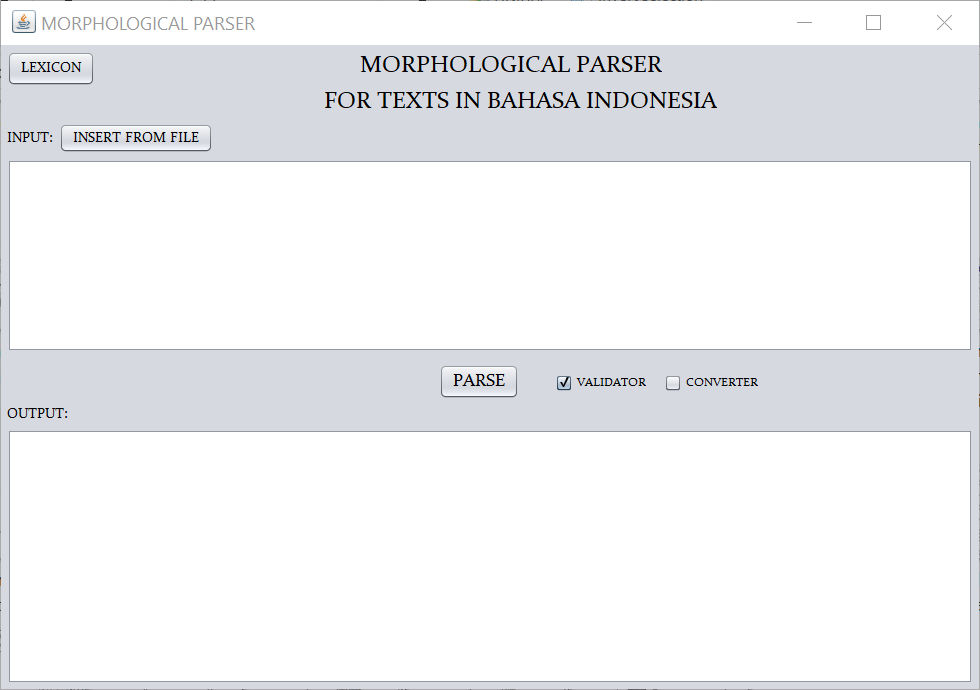
\includegraphics[scale=0.7]{Gambar/gambar-implementasi-antarmuka-parser}
\caption{Implementasi antarmuka perangkat lunak morphological parser} 
\label{gambar-implementasi-antarmuka-parser}
\end{figure}

Gambar \ref{gambar-implementasi-antarmuka-lexicon} berikut adalah implementasi antarmuka untuk perangkat lunak lexicon.

\begin{figure}[H]
\centering
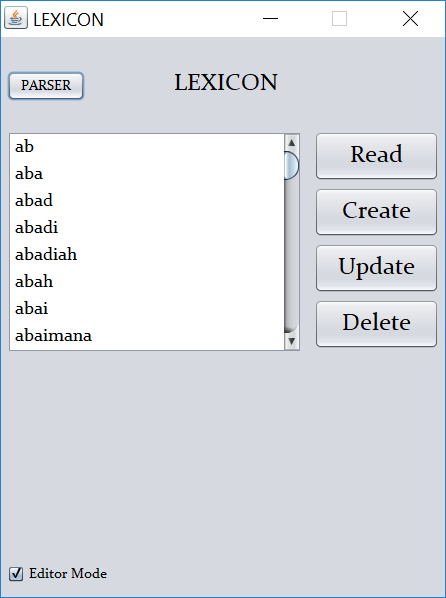
\includegraphics[scale=0.7]{Gambar/gambar-implementasi-antarmuka-lexicon}
\caption{Implementasi antarmuka perangkat lunak lexicon} 
\label{gambar-implementasi-antarmuka-lexicon}
\end{figure}

\section{Pengujian}
\label{sec:pengujian}

Pengujian yang dilakukan pada perangkat lunak yang dibuat dalam penelitian ini dibagi menjadi dua bagian. Bagian pertama merupakan pengujian fungsional yang akan menguji kesesuaian antara implementasi dari perangkat lunak dengan kebutuhan. Bagian kedua merupakan pengujian nonfungsional yang akan menguji kualitas dari perangkat lunak.

\subsection{Pengujian Fungsional}
\label{sec:pengujianFungsional}

Beberapa aspek yang akan diuji pada pengujian fungsional adalah sebagai berikut.

\begin{itemize}
	\item hasil normalisasi teks masukan
	\item hasil proses parsing
	\item proses create, update, dan delete entri leksikon
\end{itemize}

Pada tahap pengujian hasil normalisasi teks masukan dan hasil proses parsing, contoh masukan yang digunakan adalah:

\begin{itemize}
	\item Mengisi kemerdekaan Indonesia tanggal 17 Agustus adalah tanggung jawab setiap warga
	\item Ayah menyuruh, "Jangan main-main dengan makanan beku!"
\end{itemize}

Hasil normalisasi dari teks masukan tersebut adalah sebagai berikut.

\begin{itemize}
	\item mengisi kemerdekaan indonesia tanggal 17 agustus adalah tanggung jawab setiap warga
	\item ayah menyuruh jangan main-main dengan makanan beku
\end{itemize}

Hasil parsing dari kedua contoh masukan tersebut dapat dilihat pada gambar \ref{hasil-parsing-1} dan gambar \ref{hasil-parsing-2}.

\begin{figure}[H]
\centering
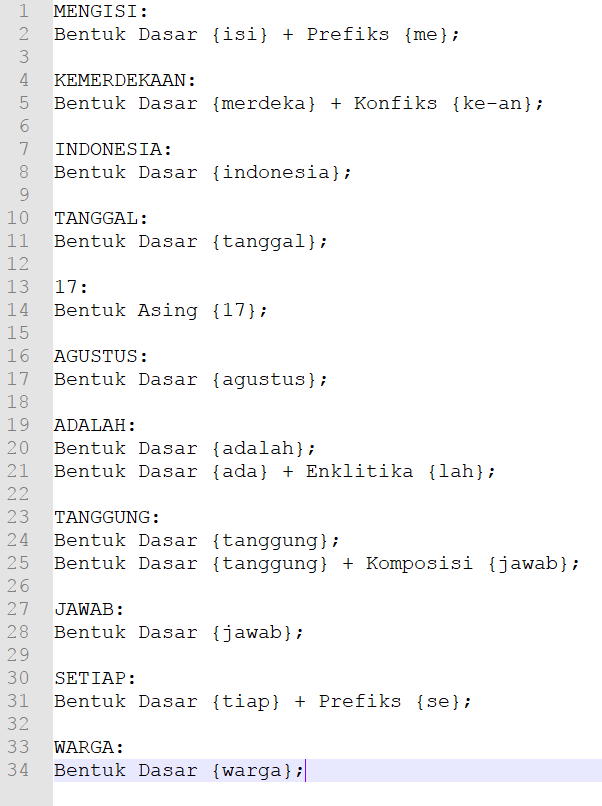
\includegraphics[scale=0.7]{Gambar/hasil-parsing-1}
\caption{Hasil parsing contoh masukan pertama} 
\label{hasil-parsing-1}
\end{figure}

\begin{figure}[H]
\centering
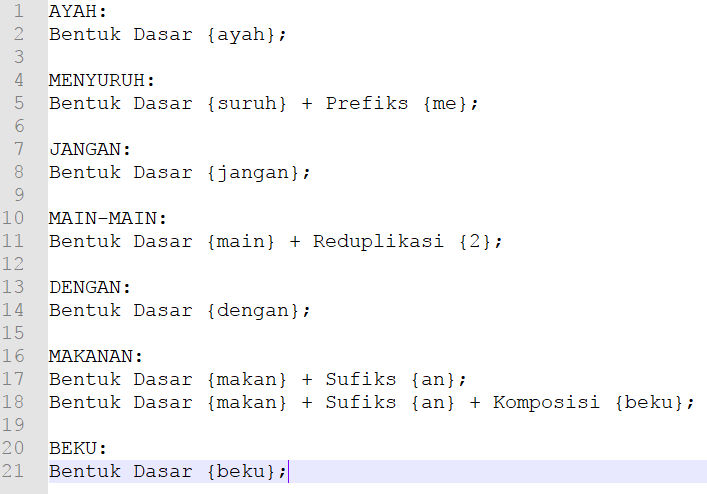
\includegraphics[scale=0.7]{Gambar/hasil-parsing-2}
\caption{Hasil parsing contoh masukan kedua} 
\label{hasil-parsing-2}
\end{figure}

Seperti dijelaskan pada subbab \ref{sec:implementasi}, perangkat lunak yang dibuat memiliki fitur untuk mengaktifkan dan mematikan fitur validator dan converter untuk memproses hasil dari proses parsing. Hasil parsing pada contoh di atas menggunakan kedua fitur validator dan converter. Hasil dari proses parsing terhadap masukan yang sama akan berbeda ketika salah satu atau kedua fitur tersebut dimatikan. Berikut adalah beberapa contoh keluaran dari masukan yang sama dengan salah satu fitur tersebut dimatikan.

Gambar \ref{hasil-parsing-tanpa-converter} berikut adalah hasil parsing dari contoh masukan pertama yang diproses tanpa fitur converter.

\begin{figure}[H]
\centering
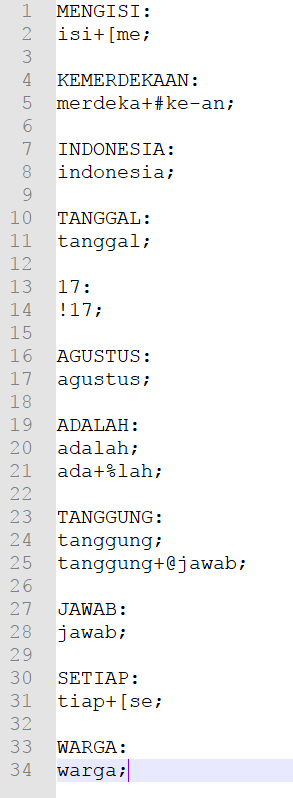
\includegraphics[scale=0.7]{Gambar/hasil-parsing-tanpa-converter}
\caption{Hasil parsing contoh masukan pertama tanpa fitur converter} 
\label{hasil-parsing-tanpa-converter}
\end{figure}

Gambar \ref{hasil-parsing-tanpa-validator} berikut adalah hasil parsing dari contoh masukan kedua yang diproses tanpa fitur validator.

\begin{figure}[H]
\centering
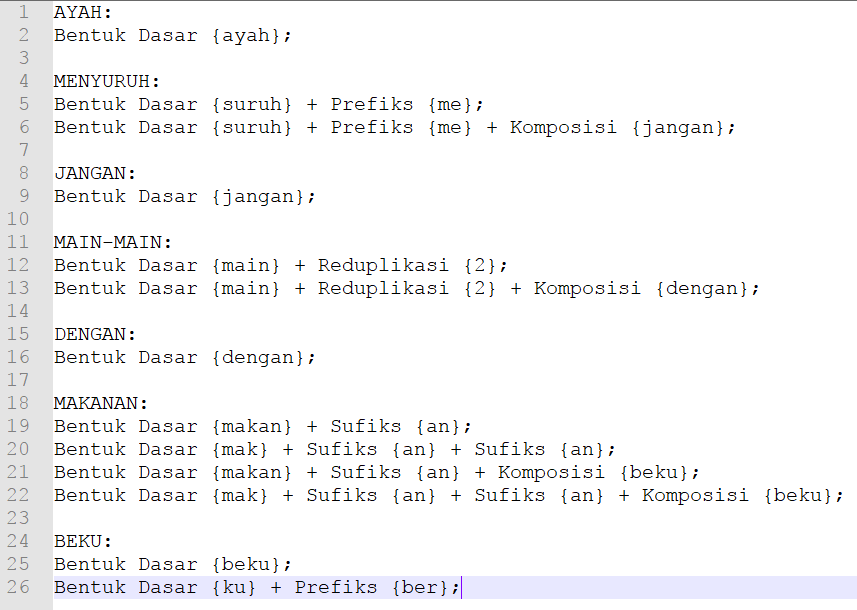
\includegraphics[scale=0.7]{Gambar/hasil-parsing-tanpa-validator}
\caption{Hasil parsing contoh masukan kedua tanpa fitur validator} 
\label{hasil-parsing-tanpa-validator}
\end{figure}

Ada beberapa jenis kata yang merupakan kata valid dalam bahasa Indonesia namun diproses secara kurang tepat dalam perangkat lunak ini, yaitu:
\begin{itemize}
	\item sekuatnya
	\item tari-menari
	\item pertama-tama
	\item ngomong-ngomong
\end{itemize}

Kata 'sekuatnya' merupakan kata yang dibentuk dari bentuk dasar $\lbrace$kuat$\rbrace$ + konfiks $\lbrace$se-nya$\rbrace$. Namun, seperti dibahas pada subbab \ref{sec:leksikon}, bentuk $\lbrace$nya$\rbrace$ dianggap sebagai klitika dan bukan dianggap sebagai sufiks dalam kesatuan konfiks $\lbrace$se-nya$\rbrace$. Oleh karena itu, kata 'sekuatnya' diproses dalam perangkat lunak menjadi bentuk dasar $\lbrace$kuat$\rbrace$ + prefiks $\lbrace$se$\rbrace$ + enklitika $\lbrace$nya$\rbrace$.

Kata 'tari-menari' merupakan contoh kata yang dibentuk dari proses reduplikasi dari bentuk dasar $\lbrace$tari$\rbrace$ lalu dilakukan proses prefiksasi, namun proses prefiksasi dilakukan bukan pada bentuk dasarnya melainkan pada kata ulangnya. Umumnya, proses reduplikasi yang diikuti proses prefiksasi pada bentuk dasar $\lbrace$tari$\rbrace$ dan prefiks $\lbrace$me$\rbrace$ akan menghasilkan kata 'menari-nari'. Sementara, pada kasus ini yang diharapkan adalah kata 'tari-menari'. Untuk bentuk kata seperti 'tari-menari' ini diproses dalam perangkat lunak seperti memproses kata ulang berubah bunyi seperti 'sayur-mayur', sehingga hasil prosesnya menjadi bentuk dasar $\lbrace$tari$\rbrace$ + reduplikasi $\lbrace$menari$\rbrace$.

Kata 'pertama-tama' merupakan contoh kata yang dibentuk dari proses reduplikasi dari bentuk dasar, namun reduplikasi tidak dilakukan secara utuh maupun berubah bunyi melainkan hanya sebagian. Sama halnya dengan bentuk 'tari-menari', bentuk ini diproses dalam perangkat lunak seperti memproses kata ulang berubah bunyi, sehingga hasil prosesnya menjadi bentuk dasar $\lbrace$pertama$\rbrace$ + reduplikasi $\lbrace$tama$\rbrace$.

Kata 'ngomong-ngomong' merupakan contoh kata yang dibentuk dari bentuk dasar $\lbrace$omong$\rbrace$ melalui proses prefiksasi dan proses reduplikasi, namun prefiks yang digunakan bukan prefiks yang baku. Prefiks yang digunakan pada bentuk ini disebut dengan prefiks nasal, seperti dijelaskan pada subbab \ref{sec:morfemAfiks}. Prefiks nasal ini tidak dapat diproses dalam perangkat lunak sehingga bentuk seperti kata 'ngomong-ngomong' dianggap sebagai bentuk asing.

Pengujian fungsional selanjutnya akan dilakukan pada proses create, update, dan delete entri leksikon, contoh masukan yang digunakan adalah:

\begin{itemize}
	\item Kata dasar 'warganet'
	\item Kata turunan 'menyayur-mayur' pada kata dasar 'sayur'
	\item Kata dasar 'abau'
\end{itemize}

Proses create akan dilakukan dengan menggunakan kata dasar 'warganet' yang merupakan serapan dari kata 'netizen' dalam bahasa Inggris. Gambar \ref{create-warganet-sebelum} berikut adalah isi dari leksikon sebelum kata tersebut dimasukkan.

\begin{figure}[H]
\centering
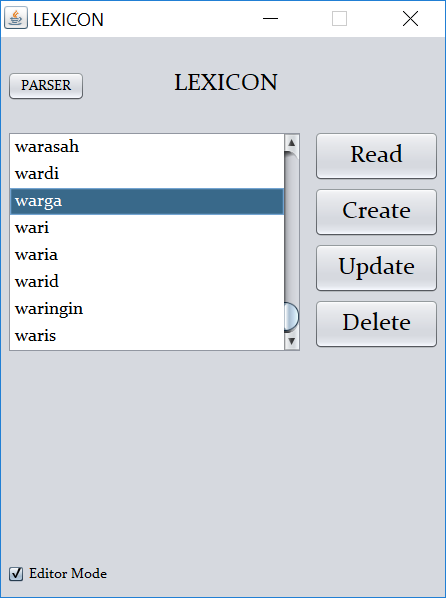
\includegraphics[scale=0.7]{Gambar/create-warganet-sebelum}
\caption{Isi leksikon sebelum kata 'warganet' dimasukkan} 
\label{create-warganet-sebelum}
\end{figure}

Gambar \ref{create-warganet-setelah} berikut adalah isi dari leksikon setelah kata 'warganet' dimasukkan.

\begin{figure}[H]
\centering
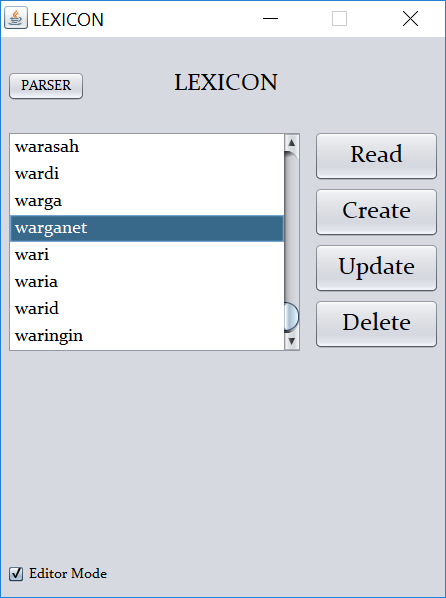
\includegraphics[scale=0.7]{Gambar/create-warganet-setelah}
\caption{Isi leksikon setelah kata 'warganet' dimasukkan} 
\label{create-warganet-setelah}
\end{figure}

Proses update akan dilakukan pada kata dasar 'sayur' dengan menambahkan kata turunan 'menyayur-mayur'. Gambar \ref{update-menyayurmayur-sebelum} berikut adalah isi dari leksikon pada kata dasar 'sayur' sebelum kata tersebut ditambahkan.

\begin{figure}[H]
\centering
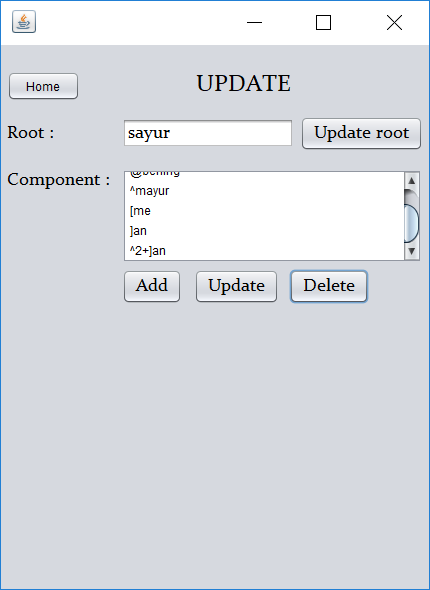
\includegraphics[scale=0.7]{Gambar/update-menyayurmayur-sebelum}
\caption{Turunan dari kata dasar 'sayur' sebelum kata turunan 'menyayur-mayur' ditambahkan} 
\label{update-menyayurmayur-sebelum}
\end{figure}

Gambar \ref{update-menyayurmayur-setelah} berikut adalah isi dari leksikon pada kata dasar 'sayur' setelah kata turunan 'menyayur-mayur' ditambahkan.

\begin{figure}[H]
\centering
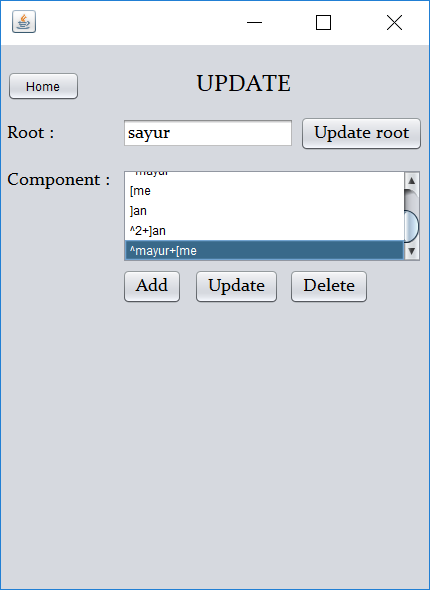
\includegraphics[scale=0.7]{Gambar/update-menyayurmayur-setelah}
\caption{Turunan dari kata dasar 'sayur' setelah kata turunan 'menyayur-mayur' ditambahkan} 
\label{update-menyayurmayur-setelah}
\end{figure}

Proses delete akan dilakukan pada kata dasar 'abau'. Gambar \ref{delete-abau-sebelum} berikut adalah isi dari leksikon sebelum kata tersebut dihapus.

\begin{figure}[H]
\centering
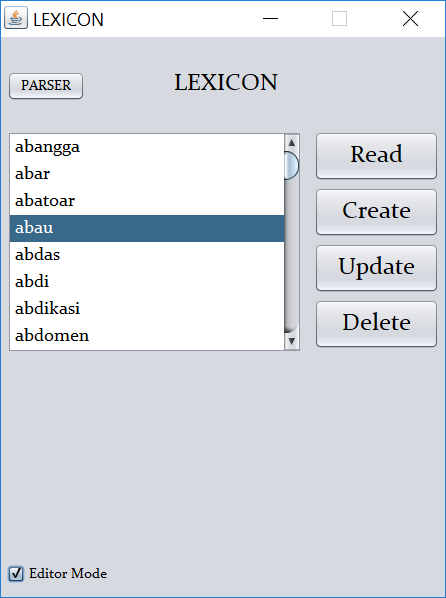
\includegraphics[scale=0.7]{Gambar/delete-abau-sebelum}
\caption{Isi leksikon sebelum kata 'abau' dihapus} 
\label{delete-abau-sebelum}
\end{figure}

Gambar \ref{delete-abau-setelah} berikut adalah isi dari leksikon setelah kata 'abau' dihapus.

\begin{figure}[H]
\centering
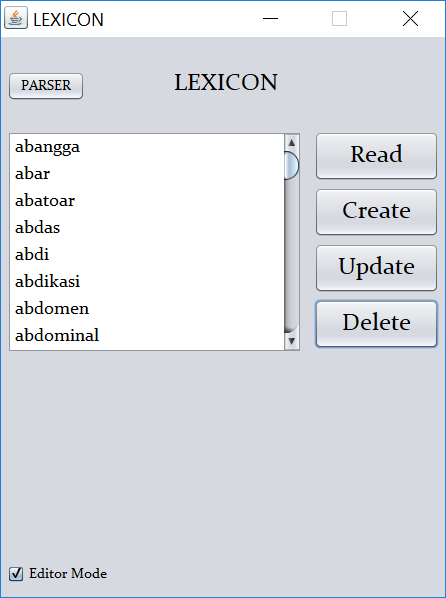
\includegraphics[scale=0.7]{Gambar/delete-abau-setelah}
\caption{Isi leksikon setelah kata 'abau' dihapus} 
\label{delete-abau-setelah}
\end{figure}

Pengujian fungsional yang dilakukan untuk beberapa aspek di atas berjalan dengan baik dan sesuai dengan yang diharapkan. Perlu dicatat, bahwa untuk menggunakan fitur validator ketika melakukan proses parsing pada perangkat lunak, supaya hasil parsing akurat dan sesuai harapan kata yang diproses harus sudah disimpan dalam leksikon, baik itu kata dasar maupun kata turunan. Pada penelitian ini, belum semua kata dasar dan kata turunan yang valid dalam bahasa Indonesia disimpan dalam leksikon. Hal ini dikarenakan ada terlalu banyak kata dalam bahasa Indonesia, khususnya kata turunan. Perangkat lunak dapat digunakan tanpa fitur validator namun hasil dari proses parsing tidak akan seakurat jika menggunakan fitur validator.

\subsection{Pengujian Nonfungsional}
\label{sec:pengujianNonfungsional}

Beberapa aspek yang akan diuji pada pengujian nonfungsional adalah sebagai berikut.

\begin{itemize}
	\item waktu yang dibutuhkan untuk melakukan proses parsing
	\item waktu yang dibutuhkan untuk melakukan create, update, dan delete entri leksikon
\end{itemize}

Pada tahap pengujian waktu proses parsing, contoh masukan yang digunakan adalah:

\begin{itemize}
	\item File txt berisi 10 kata
	\item File txt berisi 20 kata
	\item File txt berisi 100 kata
\end{itemize}

Isi file txt yang digunakan pada pengujian ini dapat dilihat pada lampiran \ref{lamp:A}.

Untuk setiap contoh masukan, dilakukan proses parsing sebanyak 5 kali dan setiap proses parsing selesai dilakukan akan dicatat waktu prosesnya. Dari data waktu proses parsing tersebut akan diambil rata-rata waktu prosesnya.

Tabel \ref{tabel-waktu-parsing-pertama} berikut berisi waktu proses parsing dan rata-ratanya untuk contoh masukan pertama.

\begin{table}[H]
\centering
\begin{tabular}{|c|c|}
\hline
\textbf{Proses ke-} & \textbf{Waktu} (dalam milidetik) \\
\hline
1&29\\
2&3\\
3&4\\
4&3\\
5&3\\
\hline
\textbf{Rata-rata} & \textbf{8,4}\\
\hline
\end{tabular}
\caption{Tabel waktu proses parsing untuk contoh masukan pertama} 
\label{tabel-waktu-parsing-pertama}
\end{table}

Tabel \ref{tabel-waktu-parsing-kedua} berikut berisi waktu proses parsing dan rata-ratanya untuk contoh masukan kedua.

\begin{table}[H]
\centering
\begin{tabular}{|c|c|}
\hline
\textbf{Proses ke-} & \textbf{Waktu} (dalam milidetik) \\
\hline
1&50\\
2&8\\
3&8\\
4&9\\
5&9\\
\hline
\textbf{Rata-rata} & \textbf{16,8}\\
\hline
\end{tabular}
\caption{Tabel waktu proses parsing untuk contoh masukan kedua} 
\label{tabel-waktu-parsing-kedua}
\end{table}

Tabel \ref{tabel-waktu-parsing-ketiga} berikut berisi waktu proses parsing dan rata-ratanya untuk contoh masukan ketiga.

\begin{table}[H]
\centering
\begin{tabular}{|c|c|}
\hline
\textbf{Proses ke-} & \textbf{Waktu} (dalam milidetik) \\
\hline
1&280\\
2&41\\
3&30\\
4&36\\
5&38\\
\hline
\textbf{Rata-rata} & \textbf{85}\\
\hline
\end{tabular}
\caption{Tabel waktu proses parsing untuk contoh masukan ketiga} 
\label{tabel-waktu-parsing-ketiga}
\end{table}

Dapat dilihat dari hasil pengujian terhadap waktu proses parsing di atas, kenaikan rata-rata waktu proses untuk contoh masukan pertama, kedua, dan ketiga berbanding lurus dengan jumlah kata yang diproses. Dapat disimpulkan bahwa waktu untuk melakukan proses parsing bergantung pada banyaknya kata yang diproses. Semakin banyak kata yang diproses waktu yang dibutuhkan untuk melakukan proses tersebut akan semakin lama.

Dapat dilihat juga pada setiap tabel waktu proses untuk setiap contoh masukan, terjadi penurunan waktu yang signifikan antara proses pertama ke proses kedua untuk proses pada contoh masukan yang sama. Dapat disimpulkan bahwa ketika dilakukan beberapa kali proses pada masukan yang sama maka waktu prosesnya akan turun cukup signifikan. Hal ini dimungkinkan karena bahasa Java menyimpan data hasil proses yang pernah dijalankan sebelumnya.

Pada tahap pengujian waktu untuk melakukan create, update, dan delete entri leksikon, akan dilakukan dengan melakukan masing-masing proses tersebut sebanyak 3 kali untuk kata yang sama. Dari data waktu proses tersebut akan diambil rata-rata waktunya.

Tabel \ref{tabel-waktu-create} berikut berisi waktu untuk melakukan create sebuah entri baru pada leksikon dan rata-ratanya.

\begin{table}[H]
\centering
\begin{tabular}{|c|c|}
\hline
\textbf{Proses ke-} & \textbf{Waktu} (dalam milidetik) \\
\hline
1&4\\
2&4\\
3&5\\
\hline
\textbf{Rata-rata} & \textbf{4,33}\\
\hline
\end{tabular}
\caption{Tabel waktu untuk melakukan create sebuah entri baru dalam leksikon} 
\label{tabel-waktu-create}
\end{table}

Tabel \ref{tabel-waktu-update} berikut berisi waktu untuk melakukan update sebuah entri pada leksikon dan rata-ratanya.

\begin{table}[H]
\centering
\begin{tabular}{|c|c|}
\hline
\textbf{Proses ke-} & \textbf{Waktu} (dalam milidetik) \\
\hline
1&7\\
2&3\\
3&2\\
\hline
\textbf{Rata-rata} & \textbf{4}\\
\hline
\end{tabular}
\caption{Tabel waktu untuk melakukan update sebuah entri dalam leksikon} 
\label{tabel-waktu-update}
\end{table}

Tabel \ref{tabel-waktu-delete} berikut berisi waktu untuk melakukan delete sebuah entri dari leksikon dan rata-ratanya.

\begin{table}[H]
\centering
\begin{tabular}{|c|c|}
\hline
\textbf{Proses ke-} & \textbf{Waktu} (dalam milidetik) \\
\hline
1&1\\
2&1\\
3&1\\
\hline
\textbf{Rata-rata} & \textbf{1}\\
\hline
\end{tabular}
\caption{Tabel waktu untuk melakukan delete sebuah entri dalam leksikon} 
\label{tabel-waktu-delete}
\end{table}

Dapat dilihat dari hasil pengujian terhadap waktu untuk melakukan create, update, dan delete entri leksikon di atas, waktu yang dibutuhkan untuk melakukan create, update, dan delete entri leksikon sangat singkat, yaitu di bawah 10 milidetik untuk setiap operasi yang dilakukan. Hal ini dikarenakan untuk melakukan operasi-operasi tersebut proses yang dilakukan adalah memodifikasi file lxc yang bersangkutan, yaitu menambahkan file baru saat melakukan create, menyisipkan kata turunan ke dalam file saat melakukan update, dan menghapus file saat melakukan delete. Proses ini sebagian besar dilakukan oleh sistem operasi dan dilakukan dengan sangat efektif.